\documentclass[11pt,a4paper]{article}

\usepackage[utf8]{inputenc}
\usepackage[T1]{fontenc}
\usepackage{lmodern}
\usepackage{geometry}
\usepackage{amsmath,amssymb,mathtools}
\usepackage{booktabs}
\usepackage{array}
\usepackage{tabularx}
\usepackage{enumitem}
\usepackage{hyperref}
\usepackage{xcolor}
\usepackage{tikz}
\usepackage{float}
\usepackage{caption}
\usepackage{microtype}
\usepackage{graphicx}
\usepackage{natbib}
\usepackage{url}

\usetikzlibrary{arrows.meta,positioning,shapes.geometric,fit,calc}
\geometry{margin=0.85in}
\hypersetup{
  colorlinks=true,
  linkcolor=blue!60!black,
  citecolor=blue!60!black,
  urlcolor=blue!60!black
}
\setlength{\parindent}{0pt}
\setlength{\parskip}{5pt}

\tikzset{
  block/.style={
    rectangle, rounded corners=3pt, draw=black!60,
    minimum width=3.0cm, minimum height=0.75cm,
    align=center, fill=gray!7, font=\small
  },
  important/.style={
    rectangle, rounded corners=3pt, draw=black!70,
    minimum width=3.2cm, minimum height=0.82cm,
    align=center, fill=blue!7, font=\small
  },
  arrow/.style={-{Latex[length=2.5mm]},thick}
}

\title{\textbf{Gap-Aware Retrieval (GAR)}\\
\large A Gap-Aware Retrieval Algorithm for Iterative Retrieval-Augmented Generation}
\author{}
\date{}

\begin{document}
\maketitle

% ============================================================
\begin{abstract}
Retrieval systems commonly rank documents according to their relevance to the original query. This can be insufficient in iterative information-seeking tasks, where the system already has some evidence and needs to retrieve only the information that is still missing. This project proposes \textbf{Gap-Aware Retrieval (GAR)}, a retrieval algorithm that uses three signals: relevance to the question and information gap, coverage of the missing information, and novelty with respect to previously collected evidence.

GAR is evaluated inside the existing MIGRES framework, which identifies missing information during iterative retrieval. MIGRES is the experimental framework; GAR is the proposed retrieval component. The surrounding MIGRES components are kept fixed as far as the original implementation permits. GAR is compared with BM25, DPR, Contriever, ColBERTv2, and SPLADE on the datasets used in the MIGRES evaluation: WikiHop, HotpotQA, MuSiQue, Natural Questions, TriviaQA, and StrategyQA.

The study evaluates retrieval quality, downstream answer quality, ablations, iteration-wise behavior, failure cases, efficiency, and statistical significance. GAR has no trainable parameters in the proposed implementation. Its scoring hyperparameters are selected on a held-out validation set using Bayesian optimization and then frozen before test evaluation. The formulation is motivated by prior work on missing-information-guided retrieval, iterative evidence coverage, relevant information gain, sentence embeddings, and efficient nearest-neighbor search \citep{wang-etal-2025-llms,yadav-etal-2020-unsupervised,pickett-etal-2024-rig,reimers-gurevych-2019-sentence,johnson-etal-2017-faiss}.
\end{abstract}

% ============================================================
\section{Introduction}

Retrieval-Augmented Generation (RAG) systems use external documents to provide a language model with information that may not be available in its parameters. A retrieval algorithm therefore has a simple but important job: given a question and a document collection, return a small set of useful documents.

A common retrieval objective is query--document relevance:
\[
q+D \longrightarrow d_1,d_2,\ldots,d_k.
\]
This works well when the question can be answered from one retrieval step. It becomes less direct when the system retrieves information iteratively. After one step, some parts of the information need may already be satisfied. The next retrieval step should focus on the remaining gap rather than repeatedly retrieving documents about the same topic.

MIGRES provides a useful setting for this problem. MIGRES is a Missing Information Guided Retrieve-Extraction-Solving framework. It identifies missing information after evidence is collected and uses that missing information to guide subsequent retrieval \citep{wang-etal-2025-llms}. In this project, we do not modify the MIGRES reasoning, extraction, or solving framework. Instead, we replace its retrieval component with GAR.

The central research question is:

\[
\boxed{\text{Does explicitly modeling the current information gap improve retrieval?}}
\]

GAR addresses this by scoring a candidate document using:
\[
\boxed{
S(d\mid q,E_t,G_t)
=
\alpha R(d,q,G_t)
+
\beta C(d,G_t)
+
\gamma N(d,E_t)
}
\]
where $R$ measures relevance, $C$ measures gap coverage, and $N$ measures evidence novelty.

The contribution of this project is the proposed GAR retrieval formulation and its controlled empirical evaluation. The individual ideas used to construct GAR are grounded in previous work; the project does not claim that semantic relevance, information coverage, or novelty are individually new.

% ============================================================
\subsection{What is MIGRES and How Does It Work?}

MIGRES stands for \textit{Missing Information Guided Retrieve-Extraction-Solving}. It is an iterative framework designed for questions that require multiple pieces of information. Instead of retrieving documents only once, MIGRES repeatedly checks what information is already available, identifies what is still missing, retrieves information for that gap, and uses the retrieved information to continue solving the question \citep{wang-etal-2025-llms}.

The basic idea is:

\[
\boxed{
\text{Question}
\rightarrow
\text{Find Missing Information}
\rightarrow
\text{Retrieve}
\rightarrow
\text{Extract}
\rightarrow
\text{Update Information}
\rightarrow
\text{Repeat if Needed}
}
\]

In simple terms, MIGRES asks three questions during the process:

\begin{enumerate}[leftmargin=1.5em]
    \item \textbf{What do we already know?}
    It keeps the evidence collected so far.

    \item \textbf{What information is still missing?}
    It identifies the missing information needed to answer the question.

    \item \textbf{What should we retrieve next?}
    It uses the missing information to guide the next retrieval step.
\end{enumerate}

For example, suppose a question requires two facts, $A$ and $B$. After the first retrieval, MIGRES may obtain $A$ but determine that $B$ is still missing. It then focuses the next retrieval step on $B$:

\[
\text{Question}
\rightarrow
\text{retrieve }A
\rightarrow
\text{missing }B
\rightarrow
\text{retrieve }B
\rightarrow
\text{answer}.
\]

MIGRES therefore maintains an iterative state consisting of the original question $q$, previously collected evidence $E_t$, and the current missing-information requirements $G_t$. These are provided to the retrieval component at each iteration:

\[
\boxed{
(q,E_t,G_t,D)
}
\]

where $D$ is the searchable document corpus.

In our work, \textbf{MIGRES is the surrounding framework, not our contribution}. We use its iterative missing-information and evidence-generation process, while replacing its retrieval component with our proposed GAR algorithm. MIGRES determines \emph{what information is missing}; GAR determines \emph{which documents are most useful for obtaining that information}.

Thus, the division of responsibility is:

\[
\boxed{
\underbrace{\text{MIGRES}}_{\text{finds what is missing}}
\rightarrow
\underbrace{\text{GAR}}_{\text{retrieves useful documents}}
\rightarrow
\underbrace{\text{MIGRES}}_{\text{extracts and updates evidence}}
}
\]

This allows us to test whether a gap-aware retrieval algorithm improves the retrieval stage while keeping the rest of the MIGRES framework unchanged.

\subsection{What We Use from MIGRES}

We use MIGRES as the surrounding experimental framework. Specifically, GAR receives the state produced by MIGRES:

\[
(q,E_t,G_t,D),
\]

where:

\begin{itemize}[leftmargin=1.5em]
\item $q$ is the original question;
\item $E_t$ is evidence collected before retrieval iteration $t$;
\item $G_t$ is the current missing-information state;
\item $D$ is the searchable document corpus.
\end{itemize}

GAR returns a ranked list of documents:

\[
T_t=\operatorname{TopK}(\mathcal{C}_t).
\]

MIGRES then continues its normal filtering, extraction, gap-analysis, and solving process.

We therefore compare:

\[
\boxed{\text{MIGRES+BM25}}
\qquad\text{vs.}\qquad
\boxed{\text{MIGRES+GAR}}.
\]

We additionally compare GAR with four other established retrieval methods.

\subsection{What We Do Not Change}

The following MIGRES components should remain fixed wherever the original implementation permits:

\begin{itemize}[leftmargin=1.5em]
\item question processing;
\item information-gap generation;
\item query-generation logic;
\item knowledge filtering;
\item information extraction;
\item answer-generation/solving model;
\item stopping conditions;
\item prompts and model settings;
\item dataset and corpus.
\end{itemize}

The main experimental variable is therefore the retrieval algorithm.

% ============================================================
\section{Information Retrieval Algorithms}

\subsection{What is an Information Retrieval Algorithm?}

An \textit{Information Retrieval (IR) algorithm} is a method used to
search a collection of documents and rank the documents according to how
useful they are for a given information need. In our setting, the
information need is represented by a question or retrieval query $q$, and
the IR algorithm produces an ordered list of documents:

\[
\boxed{
(q,D)
\rightarrow
d_1,d_2,\ldots,d_k
}
\]

where $D$ is the document collection and $d_1,\ldots,d_k$ are the top-$k$
retrieved documents.

Different IR algorithms use different signals to decide which documents
should be ranked highly. For example, BM25 primarily uses lexical
term-matching, DPR and Contriever use dense vector representations,
ColBERTv2 uses token-level late interaction, and SPLADE uses sparse neural
representations \citep{robertson-zaragoza-2009,karpukhin-etal-2020-dense,
izacard-grave-2021-contriever,santhanam-etal-2022-colbertv2,
formal-etal-2021-splade}.

In a conventional retrieval system, the main objective is:

\[
\boxed{
\text{Find documents that are relevant to the query.}
}
\]

However, in an iterative system such as MIGRES, relevance to the original
question may not be sufficient. Some information may already have been
retrieved, while other information is still missing. This motivates GAR,
which additionally considers the current information gap and the evidence
already collected.

Thus, the difference between the baseline retrieval algorithms and GAR is
not that GAR is simply another embedding model. GAR is a complete retrieval
and ranking method whose scoring function explicitly incorporates the
current information state:

\[
\boxed{
\text{Question}
+
\text{Information Gap}
+
\text{Existing Evidence}
\rightarrow
\text{Document Ranking}.
}
\]

\subsection{Why Compare Retrieval Algorithms?}

GAR is a retrieval algorithm, so the correct comparison is against established retrieval algorithms rather than against embedding models. The primary systems are:

\[
\boxed{
\text{BM25},\;
\text{DPR},\;
\text{Contriever},\;
\text{ColBERTv2},\;
\text{SPLADE},\;
\text{GAR}
}
\]

The five established methods are used through their published or official implementations where possible. GAR is implemented directly from the proposed formulation.

\subsection{BM25}

BM25 is a sparse probabilistic retrieval method based mainly on query-term frequency, inverse document frequency, and document-length normalization \citep{robertson-zaragoza-2009}.

A common form is:

\[
S_{\mathrm{BM25}}(q,d)
=
\sum_{t\in q}
IDF(t)
\frac{
f(t,d)(k_1+1)
}{
f(t,d)+k_1
\left(
1-b+b\frac{|d|}{avgdl}
\right)
}.
\]

Here $f(t,d)$ is the frequency of term $t$ in document $d$, $|d|$ is document length, $avgdl$ is average document length, and $k_1,b$ are BM25 parameters.

BM25 is especially important because it is the retrieval baseline used in the MIGRES setting.

\subsection{DPR}

Dense Passage Retrieval (DPR) uses separate dense encoders for questions and passages and retrieves documents according to their vector similarity \citep{karpukhin-etal-2020-dense}.

A simplified score is:

\[
S_{\mathrm{DPR}}(q,d)
=
\mathbf{q}^{T}\mathbf{d},
\]

where $\mathbf q$ and $\mathbf d$ are dense query and document representations.

DPR provides a supervised dense-retrieval baseline.

\subsection{Contriever}

Contriever is an unsupervised dense retrieval method based on contrastive learning \citep{izacard-grave-2021-contriever}. Its basic retrieval operation can be written as:

\[
S_{\mathrm{Contriever}}(q,d)
=
sim(\mathbf q,\mathbf d).
\]

Contriever provides a dense-retrieval baseline with a different training approach from DPR.

\subsection{ColBERTv2}

ColBERTv2 uses late interaction. Instead of representing a complete document with only one vector, it keeps token-level representations and computes efficient token-level interactions \citep{santhanam-etal-2022-colbertv2}.

A simplified score is:

\[
S_{\mathrm{ColBERT}}(q,d)
=
\sum_{i\in q}
\max_{j\in d}
sim(\mathbf q_i,\mathbf d_j).
\]

This gives a useful comparison with both single-vector dense retrieval and sparse retrieval.

\subsection{SPLADE}

SPLADE is a neural sparse retrieval method that produces sparse vocabulary representations for queries and documents \citep{formal-etal-2021-splade}.

Let:

\[
\mathbf{s}_d=f_\theta(d)
\]

be a sparse document representation. A simplified retrieval score is:

\[
S_{\mathrm{SPLADE}}(q,d)
=
\mathbf{s}_q^T\mathbf{s}_d.
\]

SPLADE provides a neural sparse baseline.

\subsection{Baseline Comparison}

\begin{center}
\begin{tabular}{lll}
\toprule
\textbf{System} & \textbf{Retrieval type} & \textbf{Role}\\
\midrule
MIGRES+BM25 & Sparse lexical & Main baseline\\
MIGRES+DPR & Dense bi-encoder & Dense baseline\\
MIGRES+Contriever & Unsupervised dense & Dense baseline\\
MIGRES+ColBERTv2 & Late interaction & Multi-vector baseline\\
MIGRES+SPLADE & Neural sparse & Neural sparse baseline\\
MIGRES+GAR & Gap-aware retrieval & Proposed method\\
\bottomrule
\end{tabular}
\end{center}

All baselines should use established implementations and published checkpoints where possible. Their exact checkpoint, index, and retrieval parameters must be recorded.

% ============================================================
\section{Development and Introduction of GAR}

\subsection{What GAR Is}

GAR is a retrieval algorithm designed for iterative retrieval. It changes the retrieval question from:

\[
\text{``Is this document relevant to the original question?''}
\]

to:

\[
\text{``Is this document useful given what is missing and what is already known?''}
\]

GAR uses three signals:

\begin{enumerate}[leftmargin=1.5em]
\item \textbf{Gap relevance}: relevance to the original question and the current information gap.
\item \textbf{Gap coverage}: how much of the missing information is covered by the candidate.
\item \textbf{Evidence novelty}: how much new information the candidate adds beyond existing evidence.
\end{enumerate}

\subsection{Why GAR Was Developed}

A query-only retriever can repeatedly return documents that are strongly related to the question but do not resolve the current missing information. MIGRES already exposes the missing-information state, making it possible for the retrieval algorithm to use that state directly \citep{wang-etal-2025-llms}.

The motivation for the GAR components comes from three sources.

First, MIGRES provides the missing-information concept: later retrieval can be targeted toward information that is still missing \citep{wang-etal-2025-llms}.

Second, Yadav et al.\ use an iterative evidence-retrieval process that focuses later retrieval on information not covered by existing justifications. This motivates the coverage component in GAR \citep{yadav-etal-2020-unsupervised}.

Third, Relevant Information Gain argues that retrieval should avoid wasting limited context on redundant information while retaining relevance \citep{pickett-etal-2024-rig}. This motivates the novelty component.

GAR combines these ideas into one retrieval score. The formulation is therefore a proposed unified model; the project does not claim that each component is independently novel.

\subsection{Applications}

GAR is intended for settings where information needs change during retrieval, including:

\begin{itemize}[leftmargin=1.5em]
\item multi-hop question answering;
\item iterative RAG;
\item research-oriented evidence retrieval;
\item evidence gathering over large document collections;
\item systems that explicitly track missing information.
\end{itemize}

GAR does not require a new language model. The surrounding system can provide the current gap and evidence state.

% ============================================================
\section{Mathematical Formulation}

\subsection{Notation}

At retrieval iteration $t$:

\[
q=\text{original question},
\]

\[
E_t=\text{evidence collected before iteration }t,
\]

\[
G_t=\{g_1,\ldots,g_m\}
\]

is the set of current information requirements, and

\[
D=\text{searchable document corpus}.
\]

A candidate document is:

\[
d\in D.
\]

An individual evidence item is:

\[
e\in E_t.
\]

The GAR input is therefore:

\[
\boxed{(q,E_t,G_t,D)}.
\]

\subsection{Text Embeddings}

GAR needs a fixed representation function:

\[
\phi:\mathcal{T}\rightarrow\mathbb{R}^{p}.
\]

We use:

\[
\boxed{
\texttt{sentence-transformers/multi-qa-mpnet-base-cos-v1}
}
\]

as the fixed embedding model. The model maps sentences and paragraphs to 768-dimensional dense vectors and was designed for semantic search \citep{reimers-gurevych-2019-sentence,multiqa-mpnet}.

The same model is used for questions, gaps, documents, and evidence. Document embeddings are computed once and stored in the ANN index.

\subsection{Cosine Similarity}

For two text items $x$ and $y$:

\[
\operatorname{cos}(x,y)
=
\frac{\phi(x)^T\phi(y)}
{\|\phi(x)\|_2\|\phi(y)\|_2}.
\]

For a normalized score in $[0,1]$, GAR uses:

\[
\boxed{
s(x,y)
=
\frac{1}{2}
\left(
1+
\frac{\phi(x)^T\phi(y)}
{\|\phi(x)\|_2\|\phi(y)\|_2}
\right)
}
\tag{1}
\]

The embedding model creates vectors; cosine similarity compares them.

\subsection{Gap Weights}

Each gap requirement has a non-negative weight:

\[
w_i\geq0,
\qquad
\sum_{i=1}^{m}w_i>0.
\]

For the first implementation:

\[
\boxed{w_i=1\quad\forall i.}
\]

This avoids introducing another learned model.

\subsection{Gap Relevance}

First calculate the weighted semantic relevance to the gap:

\[
\boxed{
s_G(d,G_t)
=
\frac{
\sum_{i=1}^{m}w_i\,s(d,g_i)
}{
\sum_{i=1}^{m}w_i
}
}
\tag{2}
\]

Then combine original-question relevance and gap relevance:

\[
\boxed{
R(d,q,G_t)
=
\lambda s(d,q)
+
(1-\lambda)s_G(d,G_t)
}
\tag{3}
\]

where:

\[
0\leq\lambda\leq1.
\]

Interpretation:

\begin{itemize}[leftmargin=1.5em]
\item $\lambda$ close to $1$: emphasize the original question;
\item $\lambda$ close to $0$: emphasize the information gap.
\end{itemize}

\subsection{Gap Coverage}

Let $\tau(x)$ be the set of normalized content tokens obtained after the fixed preprocessing pipeline.

For a non-empty gap requirement:

\[
\boxed{
c(d,g_i)
=
\frac{
|\tau(d)\cap\tau(g_i)|
}{
|\tau(g_i)|
}
}
\tag{4}
\]

This is normalized token recall. The weighted coverage score is:

\[
\boxed{
C(d,G_t)
=
\frac{
\sum_{i=1}^{m}w_i\,c(d,g_i)
}{
\sum_{i=1}^{m}w_i
}
}
\tag{5}
\]

Thus $C(d,G_t)\in[0,1]$.

If $\tau(g_i)$ is empty, that invalid requirement is removed before retrieval.

\subsection{Evidence Novelty}

For non-empty evidence:

\[
\boxed{
N(d,E_t)
=
1-\max_{e\in E_t}s(d,e)
}
\tag{6}
\]

A candidate very similar to existing evidence receives low novelty. A candidate dissimilar to all existing evidence receives high novelty.

At the first iteration:

\[
E_0=\emptyset.
\]

We define:

\[
\boxed{N(d,\emptyset)=1.}
\tag{7}
\]

\subsection{Final GAR Score}

The final score is:

\[
\boxed{
S(d\mid q,E_t,G_t)
=
\alpha R(d,q,G_t)
+
\beta C(d,G_t)
+
\gamma N(d,E_t)
}
\tag{8}
\]

subject to:

\[
\boxed{
\alpha,\beta,\gamma\geq0,
\qquad
\alpha+\beta+\gamma=1.
}
\tag{9}
\]

Because the three components are normalized, the final score is also in $[0,1]$.

\subsection{Hyperparameters}

GAR has four scoring hyperparameters:

\[
\boxed{
\alpha,\beta,\gamma,\lambda
}
\]

and one retrieval hyperparameter:

\[
\boxed{K_0}.
\]

Their roles are:

\begin{center}
\begin{tabular}{lll}
\toprule
\textbf{Parameter} & \textbf{Role} & \textbf{Constraint}\\
\midrule
$\alpha$ & Weight of relevance $R$ & $\geq0$\\
$\beta$ & Weight of coverage $C$ & $\geq0$\\
$\gamma$ & Weight of novelty $N$ & $\geq0$\\
$\lambda$ & Question-vs-gap relevance balance & $[0,1]$\\
$K_0$ & ANN candidate-pool size & $K_0\geq k$\\
\bottomrule
\end{tabular}
\end{center}

The final retrieval depth $k$ is an \textbf{experimental setting}, not a GAR-specific scoring parameter. It should be kept the same across systems for fair comparison.

The fixed embedding model and cosine similarity are also configuration choices, not learned GAR hyperparameters.

% ============================================================
\section{How GAR Works Using MIGRES}

\subsection{Overall Architecture}

\begin{center}
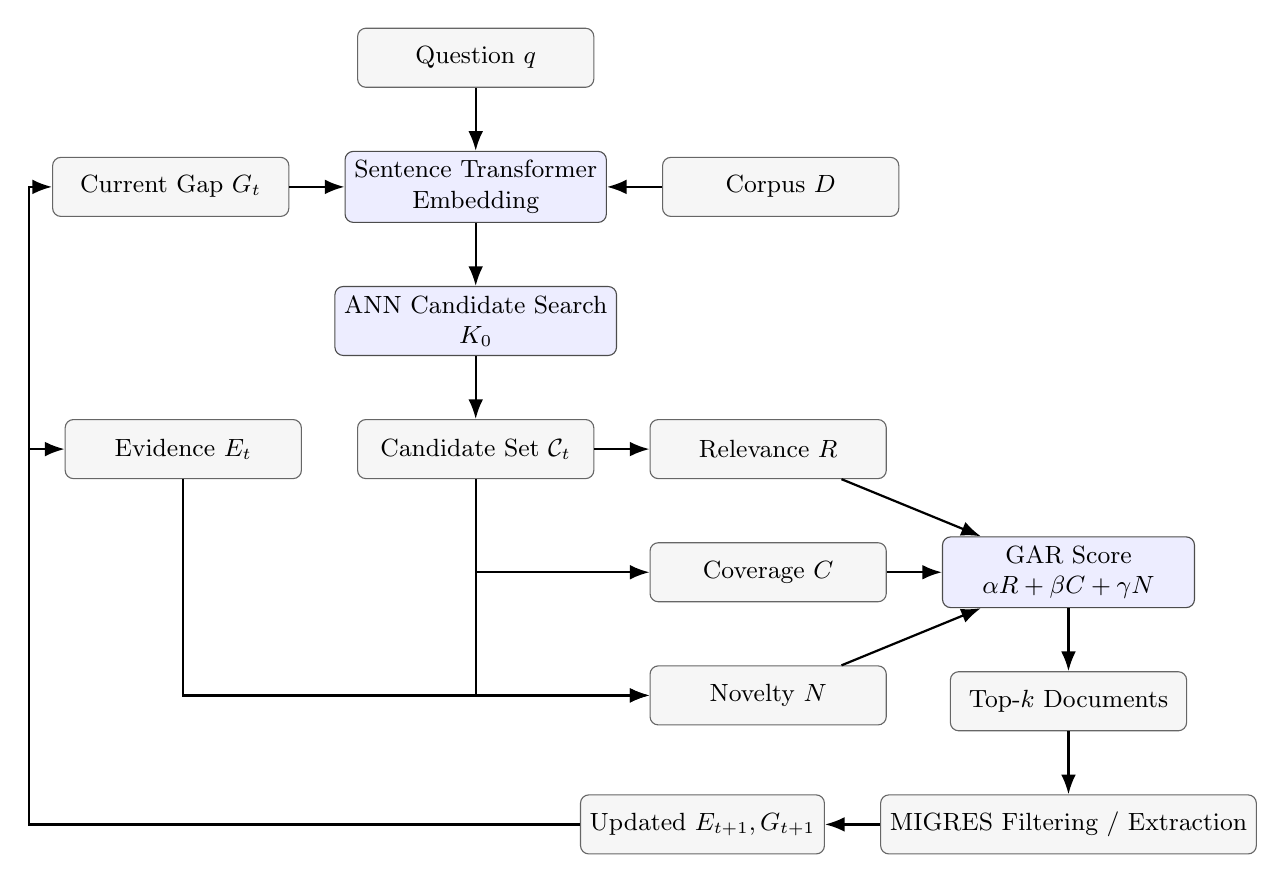
\begin{tikzpicture}[node distance=8mm and 7mm]

% Inputs
\node[block] (q) {Question $q$};

% Embedding and candidate generation
\node[important,below=of q] (emb) {Sentence Transformer\\Embedding};
\node[block,left=of emb] (g) {Current Gap $G_t$};
\node[block,right=of emb] (d) {Corpus $D$};
\node[important,below=of emb] (ann) {ANN Candidate Search\\$K_0$};
\node[block,below=of ann] (cand) {Candidate Set $\mathcal{C}_t$};
\node[block,left=of cand] (e) {Evidence $E_t$};

% GAR components
\node[block,right=of cand] (r) {Relevance $R$};
\node[block,below=of r] (c) {Coverage $C$};
\node[block,below=of c] (n) {Novelty $N$};

% Final score
\node[important,right=of c] (score)
    {GAR Score\\$\alpha R+\beta C+\gamma N$};

% Output and MIGRES
\node[block,below=of score] (top) {Top-$k$ Documents};
\node[block,below=of top] (mig) {MIGRES Filtering / Extraction};
\node[block,left=of mig] (next) {Updated $E_{t+1},G_{t+1}$};

% Input arrows
\draw[arrow] (q) -- (emb);
\draw[arrow] (g) -- (emb);
\draw[arrow] (d) -- (emb);

% Embedding -> ANN -> candidates
\draw[arrow] (emb) -- (ann);
\draw[arrow] (ann) -- (cand);

% Candidate -> each GAR component
\draw[arrow] (cand) -- (r);
\draw[arrow] (cand) |- (c);
\draw[arrow] (cand) |- (n);

% Evidence affects novelty
\draw[arrow] (e) |- (n);

% Components -> final score
\draw[arrow] (r) -- (score);
\draw[arrow] (c) -- (score);
\draw[arrow] (n) -- (score);

% Final retrieval -> MIGRES
\draw[arrow] (score) -- (top);
\draw[arrow] (top) -- (mig);

% MIGRES updates the state
\draw[arrow] (mig) -- (next);

% Feedback loop for next iteration
\draw[arrow] (next.west) -- ++(-7,0) |- (g.west);
\draw[arrow] (next.west) -- ++(-7,0) |- (e.west);

\end{tikzpicture}
\end{center}

\captionof{figure}{Overall architecture of GAR within the MIGRES framework. MIGRES provides the current question, evidence, and information gap. GAR generates candidates using ANN and ranks them using relevance, gap coverage, and evidence novelty. The retrieved documents are then returned to MIGRES for filtering, extraction, and state updating.}

\subsection{Step 1: Dataset Question}

A benchmark supplies the original question:

\[
q.
\]

The benchmark's gold answer and supporting evidence are not given to GAR during retrieval.

\subsection{Step 2: MIGRES Creates the Retrieval State}

MIGRES processes the question and maintains:

\[
E_t=\text{evidence already collected}
\]

and:

\[
G_t=\text{information still missing}.
\]

The gap can contain multiple requirements:

\[
G_t=\{g_1,\ldots,g_m\}.
\]

GAR does not independently invent $G_t$ in the main experiment. It receives the gap produced by MIGRES.

\subsection{Step 3: Convert Text to Embeddings}

GAR uses the fixed Sentence Transformer model:

\[
\phi(x).
\]

The question, each gap requirement, each document, and each evidence item can therefore be represented as vectors.

The document vectors are computed once before retrieval.

\subsection{Step 4: ANN Candidate Search}

ANN means \textbf{Approximate Nearest Neighbor}; it is not an artificial neural network.

The purpose of ANN is speed. A large corpus may contain millions of document vectors. Computing the full GAR score for every document would be unnecessarily expensive.

For each query-like input $x$, ANN returns $K_0$ nearby documents:

\[
ANN_{K_0}(x,D).
\]

GAR searches using both the original question and every gap requirement:

\[
\boxed{
\mathcal{C}_t
=
ANN_{K_0}(q,D)
\cup
\bigcup_{i=1}^{m}
ANN_{K_0}(g_i,D)
}
\tag{10}
\]

Duplicates are removed.

Thus $K_0$ is the candidate-pool size, while $k$ is the final number returned.

\subsection{Step 5: Calculate Relevance}

For every candidate:

\[
R(d,q,G_t)
\]

measures both:

\[
\text{question-document relevance}
\]

and:

\[
\text{gap-document relevance}.
\]

\subsection{Step 6: Calculate Coverage}

GAR then asks:

\[
\text{``Does this document cover the information that is missing?''}
\]

This produces:

\[
C(d,G_t).
\]

\subsection{Step 7: Calculate Novelty}

GAR then asks:

\[
\text{``Is this document redundant with evidence already collected?''}
\]

This produces:

\[
N(d,E_t).
\]

\subsection{Step 8: Calculate the GAR Score}

For every candidate:

\[
S(d\mid q,E_t,G_t)
=
\alpha R+\beta C+\gamma N.
\]

The candidate with the highest score is preferred because it is simultaneously relevant, gap-covering, and non-redundant.

\subsection{Step 9: Return Top-$k$}

GAR returns:

\[
\boxed{
T_t=
\operatorname{TopK}_{d\in\mathcal C_t}
S(d\mid q,E_t,G_t)
}
\tag{11}
\]

where $k$ is fixed for the experiment.

\subsection{Step 10: MIGRES Continues}

MIGRES receives the retrieved documents and performs its normal filtering and extraction.

It updates:

\[
E_{t+1}
\]

and, if more information is needed:

\[
G_{t+1}.
\]

GAR is then called again.

The complete loop is:

\[
\boxed{
(q,E_t,G_t,D)
\xrightarrow{\mathrm{GAR}}
T_t
\xrightarrow{\mathrm{MIGRES}}
(E_{t+1},G_{t+1})
\xrightarrow{\mathrm{GAR}}
T_{t+1}
}
\]

This is why GAR is evaluated inside MIGRES rather than as an isolated one-shot retriever.

\subsection{Candidate Generation vs.\ GAR Ranking}

The two stages must not be confused:

\[
\boxed{
\text{Embedding}
\rightarrow
\text{ANN candidate generation}
\rightarrow
\text{GAR scoring}
\rightarrow
\text{Top-}k
}
\]

Embedding creates vectors.

ANN finds a manageable candidate set.

GAR makes the final ranking decision.

If BM25 is used to create the candidate pool and GAR only reranks those documents, that is a \emph{GAR reranker} experiment, not the complete GAR retrieval experiment proposed here.

% ============================================================
\subsection{Development, Validation, and Test Protocol}

\subsubsection{Is GAR Trained?}

No.

The proposed GAR algorithm has no trainable parameters. We do not train GAR on $D_{\mathrm{train}}$.

The embedding model is a fixed pretrained Sentence Transformer. It is not fine-tuned in the primary experiment.

Therefore the experiment has no GAR training stage.

\subsubsection{Training Data}

If a baseline uses an official pretrained checkpoint, we use that checkpoint rather than retraining it on the evaluation data.

The benchmark training split may be used for auxiliary development or baseline-specific training only if required by the official implementation. Any such use must be documented and must not use test annotations.

For GAR itself:

\[
D_{\mathrm{train}}
\not\rightarrow
\text{GAR parameter learning}.
\]

\subsubsection{Validation Set $D_{\mathrm{val}}$}

We define:

\[
\boxed{D_{\mathrm{val}}=\text{the held-out development/validation split}.}
\]

Where an official development split exists, we use it. The exact files and split names are recorded for each dataset.

GAR hyperparameters are selected using the \emph{complete MIGRES+GAR pipeline} on $D_{\mathrm{val}}$.

This is important because GAR cannot be meaningfully validated in isolation: $E_t$ and $G_t$ are produced by the MIGRES iterative process.

The validation loop is:

\[
D_{\mathrm{val}}
\rightarrow
\text{MIGRES}
\rightarrow
(q,E_t,G_t)
\rightarrow
\text{GAR}
\rightarrow
\text{MIGRES}
\rightarrow
\text{validation metric}.
\]

\subsubsection{Bayesian Optimization}

We use Bayesian optimization to select:

\[
\theta_{\mathrm{GAR}}
=
\{\alpha,\beta,\gamma,\lambda,K_0\}.
\]

Bayesian optimization uses previous validation evaluations to decide which configuration to test next rather than exhaustively evaluating every possible combination \citep{snoek2012practical}.

The search space is:

\[
\alpha,\beta,\gamma\geq0,
\qquad
\alpha+\beta+\gamma=1,
\]

\[
0\leq\lambda\leq1,
\]

and a predefined discrete candidate set for $K_0$, for example:

\[
K_0\in\{50,100,200,500\}.
\]

The exact search space and random seed are recorded before the experiment.

The optimization objective must be selected before test evaluation. The primary objective should be a retrieval metric aligned with the main research question, such as Recall@$k$ on $D_{\mathrm{val}}$.

The procedure is:

\[
\boxed{
D_{\mathrm{val}}
\rightarrow
\text{MIGRES+GAR}
\rightarrow
\text{validation score}
\rightarrow
\text{Bayesian optimization}
\rightarrow
\theta^*_{\mathrm{GAR}}
}
\]

The selected configuration is then frozen.

\subsubsection{Test Set $D_{\mathrm{test}}$}

After validation:

\[
\boxed{
\theta^*_{\mathrm{GAR}}
\text{ is frozen.}
}
\]

We then evaluate:

\[
D_{\mathrm{test}}
\rightarrow
\text{MIGRES+GAR}(\theta^*_{\mathrm{GAR}})
\rightarrow
\text{final metrics}.
\]

No test result is used to change the hyperparameters.

The same $k$, dataset, corpus, MIGRES configuration, and stopping conditions are used for the comparison systems wherever possible.

\subsubsection{Complete Experimental Flow}

\begin{enumerate}[leftmargin=1.5em]
\item Prepare the official dataset splits and searchable corpus.
\item Reproduce MIGRES+BM25.
\item Verify the MIGRES retrieval interface and confirm how $E_t$ and $G_t$ are exposed.
\item Build the fixed GAR document embeddings.
\item Build the ANN index.
\item Implement and unit-test the GAR equations.
\item Run Bayesian optimization on $D_{\mathrm{val}}$ through the complete MIGRES+GAR pipeline.
\item Freeze $\alpha,\beta,\gamma,\lambda,K_0$.
\item Run the held-out $D_{\mathrm{test}}$ with the frozen configuration.
\item Run BM25, DPR, Contriever, ColBERTv2, and SPLADE using their established implementations.
\item Evaluate retrieval quality, downstream answer quality, efficiency, and cost.
\item Run GAR ablations using the same frozen evaluation protocol.
\end{enumerate}

% ============================================================
\section{Datasets}

\subsection{Dataset Selection}

The project uses the six datasets reported in the MIGRES evaluation:

\[
\boxed{
\text{WikiHop},\;
\text{HotpotQA},\;
\text{MuSiQue},\;
\text{Natural Questions},\;
\text{TriviaQA},\;
\text{StrategyQA}
}
\]

These datasets provide questions and task-specific answer/evidence annotations suitable for evaluating retrieval and downstream question answering.

\subsection{WikiHop}

\textbf{Paper:} \citet{welbl-etal-2018-constructing}.

WikiHop is a multi-document, multi-hop reading-comprehension benchmark designed so that the answer requires combining information across documents. The dataset is useful for GAR because it tests whether retrieval can assemble complementary evidence rather than repeatedly retrieving one topic.

Typical fields include a question, candidate documents, an answer, and supporting information.

Paper:
\url{https://aclanthology.org/Q18-1021/}

\subsection{HotpotQA}

\textbf{Paper:} \citet{yang-etal-2018-hotpotqa}.

HotpotQA contains about 113K Wikipedia-based question-answer pairs and provides sentence-level supporting facts. It includes multi-hop and comparison questions \citep{yang-etal-2018-hotpotqa}.

For first-stage development, we use the FullWiki setting because it requires retrieval from a larger Wikipedia corpus. The official repository provides train, development, and FullWiki resources and explicitly allows researchers to replace its retrieval component with their own IR system.

Paper:
\url{https://aclanthology.org/D18-1259/}

Official resources:
\url{https://hotpotqa.github.io/}

The repository documentation describes the FullWiki development and test files and the use of custom IR systems.

\subsection{MuSiQue}

\textbf{Paper:} \citet{trivedi-etal-2022-musique}.

MuSiQue was designed to reduce shortcut solutions in multi-hop QA. MuSiQue-Ans contains about 25K questions requiring 2--4 hops \citep{trivedi-etal-2022-musique}.

Typical information includes a question, answer, reasoning structure, and supporting evidence.

Paper:
\url{https://aclanthology.org/2022.tacl-1.31/}

Official repository:
\url{https://github.com/StonyBrookNLP/musique}

\subsection{Natural Questions}

\textbf{Paper:} \citet{kwiatkowski-etal-2019-natural}.

Natural Questions consists of real anonymized queries issued to Google Search and Wikipedia-based annotations. The public release contains 307,373 training examples, 7,830 development examples, and 7,842 sequestered test examples \citep{kwiatkowski-etal-2019-natural}.

Typical fields include a question, Wikipedia page information, long-answer annotations, short-answer annotations, and document-level information.

Paper:
\url{https://aclanthology.org/Q19-1026/}

Official research page:
\url{https://ai.google/research/NaturalQuestions}

\subsection{TriviaQA}

\textbf{Paper:} \citet{joshi-etal-2017-triviaqa}.

TriviaQA contains about 95K question-answer pairs and more than 650K question-answer-evidence triples. Questions were written by trivia enthusiasts and paired with independently gathered evidence documents \citep{joshi-etal-2017-triviaqa}.

Typical fields include a question, answer, aliases, and evidence documents.

Paper:
\url{https://aclanthology.org/P17-1147/}

Official resources:
\url{https://nlp.cs.washington.edu/triviaqa/}

\subsection{StrategyQA}

\textbf{Paper:} \citet{geva-etal-2021-strategyqa}.

StrategyQA contains 2,780 questions with implicit reasoning strategies. Each example includes a question, a reasoning decomposition, and Wikipedia evidence paragraphs \citep{geva-etal-2021-strategyqa}.

This makes it useful for testing whether gap-aware retrieval helps when the required reasoning steps are not directly stated in the question.

Paper:
\url{https://aclanthology.org/2021.tacl-1.21/}

Official resources:
\url{https://allenai.org/data/strategyqa}

\subsection{Dataset Summary}

\begin{center}
\small
\begin{tabular}{p{2.7cm}p{2.5cm}p{7.3cm}}
\toprule
\textbf{Dataset} & \textbf{Scale} & \textbf{Useful properties for GAR}\\
\midrule
WikiHop & $\sim$51K & Multi-document, multi-hop reasoning.\\
HotpotQA & $\sim$113K & Multi-hop QA with sentence-level supporting facts; FullWiki retrieval.\\
MuSiQue & $\sim$25K & 2--4 hop compositional reasoning.\\
Natural Questions & 307,373 train; 7,830 dev; 7,842 test & Real search questions with Wikipedia annotations.\\
TriviaQA & $\sim$95K QA pairs; $>$650K evidence triples & Heterogeneous evidence and lexical variation.\\
StrategyQA & 2,780 & Implicit reasoning with evidence paragraphs.\\
\bottomrule
\end{tabular}
\end{center}

Exact counts used in experiments must be taken from the downloaded release and recorded in the experiment configuration. Dataset counts can differ by release or preprocessing.

\subsection{What a Dataset Example Looks Like}

The common conceptual structure is:

\[
\boxed{
\text{Question}
+
\text{Corpus/Evidence}
+
\text{Answer}
+
\text{Ground-Truth Evidence/Annotations}
}
\]

For example, a HotpotQA-style example contains a natural-language question, an answer, supporting facts, and Wikipedia context. During retrieval, GAR receives the question and searchable corpus through MIGRES. The gold answer and gold supporting evidence are reserved for evaluation.

The ground-truth evidence must never be used to construct $G_t$, $E_t$, or the ANN candidate pool during test-time retrieval.

\subsection{Dataset Split Policy}

For each dataset:

\[
D_{\mathrm{train}},\quad
D_{\mathrm{val}},\quad
D_{\mathrm{test}}
\]

are treated separately where official splits are available.

For GAR:

\[
D_{\mathrm{val}}
\]

is used for hyperparameter optimization, while:

\[
D_{\mathrm{test}}
\]

is used only for the final evaluation.

If an official public test set has hidden answers, its evaluation follows the dataset's official evaluation procedure.

% ============================================================
\section{Experiments}

\subsection{Research Questions}

\textbf{RQ1.} Does GAR improve retrieval quality over the MIGRES BM25 baseline?

\[
\boxed{
\text{MIGRES+GAR}
\;>\;
\text{MIGRES+BM25}?
}
\]

\textbf{RQ2.} Does GAR outperform strong dense, sparse, and late-interaction retrieval methods?

\[
\text{GAR}
\quad\text{vs.}\quad
\{\text{DPR, Contriever, ColBERTv2, SPLADE}\}.
\]

\textbf{RQ3.} Does replacing BM25 with GAR improve downstream MIGRES answer quality?

\textbf{RQ4.} Which GAR component contributes most: relevance, coverage, or novelty?

\textbf{RQ5.} Does GAR generalize across the six datasets?

\textbf{RQ6.} What is the computational cost of GAR compared with the baselines?

\textbf{RQ7.} Does GAR improve retrieval without adding unnecessary LLM calls?

\textbf{RQ8.} How does GAR's retrieval effectiveness and evidence selection behavior change across successive MIGRES retrieval iterations?

\textbf{RQ9.} What are the main failure modes of GAR, and at which stage of the retrieval pipeline do these failures occur?

RQ8 is investigated through iteration-wise analysis of retrieval effectiveness and the retrieved evidence as the MIGRES state changes. RQ9 is investigated through failure-case analysis and candidate-pool diagnostics. These analyses are diagnostic and do not add a new scoring component, trainable model, or GAR hyperparameter.

\subsection{Hypotheses}

Primary hypothesis:

\[
H_0:\quad
\text{GAR does not improve retrieval performance over BM25.}
\]

\[
H_1:\quad
\text{GAR improves retrieval performance over BM25.}
\]

Secondary hypothesis:

\[
H_0:\quad
\text{GAR}\leq\text{best baseline}.
\]

\[
H_1:\quad
\text{GAR}>\text{best baseline}.
\]

For ablations:

\[
H_0:\quad
\text{removing a GAR component does not change performance}.
\]

\[
H_1:\quad
\text{removing a GAR component reduces performance}.
\]

We report effect sizes and confidence intervals together with statistical significance. The exact paired statistical test should be fixed before inspecting the final test results; a paired bootstrap or paired permutation procedure is suitable for per-question retrieval metrics.

\subsection{Main Comparison}

The main experiment compares:

\[
\boxed{
\begin{array}{c}
\text{MIGRES+BM25}\\
\text{MIGRES+DPR}\\
\text{MIGRES+Contriever}\\
\text{MIGRES+ColBERTv2}\\
\text{MIGRES+SPLADE}\\
\text{MIGRES+GAR}
\end{array}
}
\]

The same questions, corpus, $k$, MIGRES settings, answer-generation model, and stopping conditions should be used wherever possible.

\subsection{Ablation Studies}

The full GAR model is:

\[
S_{\mathrm{GAR}}
=
\alpha R+\beta C+\gamma N.
\]

We remove one component at a time.

Without relevance:

\[
\boxed{
S_{-R}(d)
=
\beta C(d,G_t)+\gamma N(d,E_t)
}
\]

Without coverage:

\[
\boxed{
S_{-C}(d)
=
\alpha R(d,q,G_t)+\gamma N(d,E_t)
}
\]

Without novelty:

\[
\boxed{
S_{-N}(d)
=
\alpha R(d,q,G_t)+\beta C(d,G_t)
}
\]

We also recommend two additional diagnostic ablations:

\[
GAR_{\mathrm{Q-only}}
\]

which uses only question relevance, and:

\[
GAR_{\mathrm{Q+G}}
\]

which uses question and gap relevance but not novelty.

These help determine whether the main benefit comes from simply adding the gap representation or from the complete relevance--coverage--novelty combination.

\subsection{Candidate-Pool Sensitivity}

Because $K_0$ controls how many candidates reach the full GAR scorer, we test:

\[
K_0\in\{50,100,200,500\}
\]

on the validation set during optimization.

The test experiment uses only the selected value.

We report both retrieval quality and latency as $K_0$ changes. We also record whether ground-truth relevant evidence is present in the ANN candidate set. This separates candidate-generation failures from GAR ranking failures.

\subsection{Iteration-Wise Analysis}

Because GAR is designed for iterative retrieval, retrieval behavior is analyzed separately across successive MIGRES iterations. We compare retrieval effectiveness in the first iteration with later iterations, where previously collected evidence and the current information gap are available to GAR.

The analysis examines whether later retrieval steps provide more complementary evidence and whether the practical contribution of relevance, coverage, and novelty changes as the evidence state evolves. This is an analysis of the existing GAR formulation and does not introduce additional parameters.

\subsection{Failure-Case Analysis}

We perform error analysis on questions where GAR fails to retrieve required evidence or does not improve the final answer. Failure cases are categorized by the stage responsible for the observed problem:

\begin{itemize}[leftmargin=1.5em]
\item incorrect or incomplete information gaps generated by MIGRES;
\item semantic mismatch between useful evidence and the embedding representation;
\item insufficient gap coverage despite high relevance;
\item useful evidence receiving a low novelty score because it is similar to existing evidence;
\item relevant evidence being absent from the ANN candidate pool;
\item multi-hop cases where a document becomes useful only after another evidence item has been collected.
\end{itemize}

The purpose is to identify the conditions under which GAR succeeds or fails rather than to modify the primary retrieval formulation.

\subsection{Gap-Coverage Diagnostic}

GAR currently measures gap coverage using normalized lexical token overlap. We retain this formulation in the primary experiment.

As a diagnostic, we inspect cases where lexical overlap and actual evidence usefulness appear to disagree. This helps determine whether token overlap is a reasonable approximation of information-gap coverage and identifies a concrete limitation for future work without introducing a second coverage model into the main experiment.

\subsection{Retrieval Metrics}

\subsubsection{Recall@$k$}

Recall@$k$ measures how much of the ground-truth relevant evidence appears in the first $k$ retrieved documents:

\[
\boxed{
Recall@k
=
\frac{
|\text{relevant evidence}\cap\text{top-}k|
}{
|\text{relevant evidence}|
}
}
\]

This is a primary metric because GAR is designed to retrieve missing evidence.

\subsubsection{Precision@$k$}

\[
\boxed{
Precision@k
=
\frac{
|\text{relevant documents in top-}k|
}{
k
}
}
\]

Precision measures how much of the retrieved set is relevant.

\subsubsection{MRR}

Mean Reciprocal Rank measures how early the first relevant result appears:

\[
\boxed{
MRR
=
\frac{1}{N}
\sum_{i=1}^{N}
\frac{1}{rank_i}
}
\]

where $rank_i$ is the rank of the first relevant result for question $i$.

\subsubsection{nDCG@$k$}

For graded relevance:

\[
DCG@k
=
\sum_{i=1}^{k}
\frac{2^{rel_i}-1}{\log_2(i+1)}
\]

and:

\[
\boxed{
nDCG@k
=
\frac{DCG@k}{IDCG@k}
}
\]

where $IDCG@k$ is the ideal DCG at cutoff $k$ \citep{jarvelin-kekalainen-2002}.

\subsubsection{Evidence Coverage}

Because GAR explicitly models an information gap, we additionally report an evidence-coverage measure where the dataset annotations permit it:

\[
\boxed{
GapEvidenceCoverage@k
=
\frac{
\text{ground-truth evidence requirements retrieved in top-}k
}{
\text{total ground-truth evidence requirements}
}
}
\]

The exact mapping from benchmark annotations to evidence requirements must be defined separately for each dataset.

\subsection{Downstream QA Metrics}

The final MIGRES answer is evaluated using the metrics supported by each benchmark.

These may include:

\begin{itemize}[leftmargin=1.5em]
\item Exact Match (EM);
\item token-level F1;
\item answer accuracy for classification-style datasets;
\item evidence/supporting-fact quality where annotations permit.
\end{itemize}

For a benchmark with a normalized answer set $A_i$:

\[
EM_i=
\mathbb{1}[\hat a_i\in A_i].
\]

Average exact match is:

\[
EM=
\frac{1}{N}
\sum_{i=1}^{N}EM_i.
\]

For token-level F1, precision and recall are computed over normalized answer tokens and then combined as:

\[
F1=\frac{2PR}{P+R}.
\]

The benchmark's official evaluation script should be used whenever available.

\subsection{Efficiency Metrics}

We report:

\begin{itemize}[leftmargin=1.5em]
\item retrieval latency per question;
\item ANN indexing time;
\item index memory;
\item number of retrieval iterations;
\item number of documents scored by GAR;
\item number of LLM calls in the complete MIGRES system;
\item input and output tokens;
\item API cost where applicable.
\end{itemize}

The GAR scorer itself should not require one LLM call per candidate. Embeddings, cosine similarity, lexical coverage, and novelty can be calculated locally.

\subsection{API Cost}

If an external model is used by MIGRES, the cost for question $q$ is:

\[
\boxed{
Cost(q)
=
T_{\mathrm{in}}(q)p_{\mathrm{in}}
+
T_{\mathrm{out}}(q)p_{\mathrm{out}}
}
\]

where $T_{\mathrm{in}}$ and $T_{\mathrm{out}}$ are input and output token counts and $p_{\mathrm{in}},p_{\mathrm{out}}$ are the corresponding prices.

Average cost is:

\[
\boxed{
\overline{Cost}
=
\frac{1}{N}
\sum_{i=1}^{N}Cost(q_i)
}
\]

The comparison must distinguish GAR's local retrieval computation from the LLM cost of the surrounding MIGRES framework.

\subsection{Fairness Controls}

The following should remain fixed across systems:

\begin{itemize}[leftmargin=1.5em]
\item dataset split;
\item question set;
\item document corpus;
\item final retrieval depth $k$;
\item MIGRES components outside retrieval;
\item answer-generation model;
\item stopping conditions;
\item evaluation scripts;
\item random seeds where applicable.
\end{itemize}

Only the retrieval method should change.

\subsection{Reproducibility Configuration}

The final experiment record should contain:

\begin{center}
\begin{tabular}{ll}
\toprule
\textbf{Parameter} & \textbf{Value}\\
\midrule
Dataset & Exact release and split\\
Corpus & Exact corpus version\\
Retriever & BM25 / DPR / Contriever / ColBERTv2 / SPLADE / GAR\\
Baseline checkpoint & Exact model/checkpoint\\
GAR embedding model & \texttt{multi-qa-mpnet-base-cos-v1}\\
Final retrieval depth $k$ & Fixed value for all systems\\
ANN candidate pool $K_0$ & Validation-selected GAR value\\
$\alpha$ & Validation-selected value\\
$\beta$ & Validation-selected value\\
$\gamma$ & Validation-selected value\\
$\lambda$ & Validation-selected value\\
Bayesian optimization seed & Recorded value\\
ANN implementation & Exact library/index\\
Hardware & CPU/GPU configuration\\
Software & Python and package versions\\
MIGRES configuration & Exact prompts/model/settings\\
\bottomrule
\end{tabular}
\end{center}

% ============================================================
\section{Conclusion}

This project proposes Gap-Aware Retrieval (GAR) as a retrieval algorithm for iterative information-seeking systems. GAR is evaluated inside MIGRES rather than replacing the MIGRES framework itself.

The core idea is:

\[
\boxed{
\text{Relevant}
+
\text{Gap-covering}
+
\text{Non-redundant}
}
\]

implemented as:

\[
\boxed{
S(d\mid q,E_t,G_t)
=
\alpha R(d,q,G_t)
+
\beta C(d,G_t)
+
\gamma N(d,E_t)
}
\]

The complete retrieval pipeline is:

\[
\boxed{
\text{Sentence Transformer}
\rightarrow
\text{Cosine Similarity}
\rightarrow
\text{ANN Candidate Search}
\rightarrow
\text{GAR Scoring}
\rightarrow
\text{Top-}k
\rightarrow
\text{MIGRES}
}
\]

GAR has no training stage in the primary experiment. Its scoring hyperparameters are selected on $D_{\mathrm{val}}$ through the complete MIGRES+GAR pipeline using Bayesian optimization and then frozen for $D_{\mathrm{test}}$.

The central empirical question is whether using the information gap and previously collected evidence produces more useful retrieval than standard retrieval algorithms. The study also examines how this behavior changes across retrieval iterations and identifies the principal failure modes of the proposed retrieval pipeline.

% ============================================================
\bibliographystyle{unsrtnat}
\bibliography{gar_references}

\end{document}
